\documentclass[a4paper,oneside]{book}

% Egy hasznos Mac OS X-es videó:
% http://www.youtube.com/watch?v=XFiLjB9UNaA&feature=related

% Oyepa, Working Tagged Filesystem:
% http://pages.stern.nyu.edu/~marriaga/software/oyepa/

\usepackage{tdk}

\usepackage{listings}
\usepackage{tikz}

\usepackage{rotating}


\usepackage{color}
\usepackage{soulutf8}
\definecolor{comment}{rgb}{0,0.6,0.2}

\usepackage{CJKutf8}
\usepackage{graphicx}
\usepackage[utf8]{inputenc}
\usepackage{marginnote}
\usepackage{listings}
\graphicspath{ {../dolgozat/images/} }


% Code colorature
\definecolor{paszt}{RGB}{252,252,252}
\definecolor{keret}{RGB}{220,220,220}
\lstset{
backgroundcolor=\color{paszt},
% showlines=true,
framexleftmargin=4mm,
framexrightmargin=4mm,
framextopmargin=2mm,
framexbottommargin=2mm,
frameround=tttt,
frame=trbl,
rulecolor=\color{keret},
extendedchars=true,
literate={á}{{\'a}}1 {é}{{\'e}}1 {ö}{{\"o}}1 {ő}{{\H{o}}}1 {ó}{{\'o}}1,
%inputencoding=utf8
}

% Line spacing (1.5-ös sorköz)
\linespread{1.2}

% Set spacing in source code (normál sorköz -1.5)
%\lstset{
%lineskip={-3pt}
%}

\usepackage{pslatex}

%%% Font settings
% \usepackage{times}
\usepackage{lmodern} % !!!
% \usepackage{chancery}
% \usepackage{charter}
% \usepackage{palatino}
% \usepackage{mathpazo}
% \usepackage{mathpple} % !!!
% \usepackage{mathptmx}

\usepackage{pstricks}

\usepackage{cpp}
\usepackage{python}

% Colors
\usepackage{color}

% Task
\newenvironment{comment}[1]
{\color{green}\noindent{$\circ$ \textit{#1}}

\smallskip

\color{gray}

}{\bigskip}

\begin{document}

% \pagestyle{empty} %a címlapon ne legyen semmi=empty, azaz nincs fejléc és lábléc

% Címlap
\begin{center}
\begin{tabular*}{\hsize}{@{}c@{\extracolsep{\fill}}c@{\extracolsep{\fill}}c@{}}
\multirow{2}[4]*{
\epsfig{file=images/ME_logo.eps,height=2truecm}}& \textcolor{blue}{\large\bfseries MISKOLCI EGYETEM}&\multirow{2}[4]*{
\epsfig{file=images/gepesz_logo.eps,height=1.6truecm}}\\
&\textcolor{blue}{\large\bfseries GÉPÉSZMÉRNÖKI ÉS INFORMATIKAI KAR}&\\
\end{tabular*}
\end{center}

\vglue 2.5truecm %függleges helykihagyás

\pagestyle{empty}

%A szakdolgozat címe, akár több sorban is
{\LARGE
\begin{center}
\textcolor{blue}{\Large\bfseries TDK DOLGOZAT}
\end{center}}

\vspace*{2.5truecm}
\begin{center}
% (Tag Based Document Management)
\LARGE\bfseries Kínai karakterek felismerése \\
generált minták alapján
\end{center}
\vglue 2cm

{\large
\begin{center}
\begin{tabular}{c}
{\bfseries Szilvási Péter}\\
Mérnökinformatikus BSc
\end{tabular}
\end{center}
\vglue 3cm
\begin{center}
\textbf{Konzulens:}
\end{center}
\medskip
\begin{center}
\begin{tabular}{ccc}
\textbf{Piller Imre} \\
tanársegéd \\
Alkalmazott Matematikai Intézeti Tanszék \\
\end{tabular}
\end{center}
\vfill
{\large

\begin{center}
\textbf{\textsc{Miskolc, 2018}}
\end{center}}

\newpage


% Font size
% \large

% Tartalomjegyzék
\tableofcontents
\thispagestyle{empty}
\cleardoublepage

% Set page style !!!
\pagestyle{fancy}

% Set number of page
\setcounter{page}{1}

% Chapters
\Chapter{Bevezetés}

A Mesterséges Intelligencia (MI) kutatás napjaink egyik legdinamikusabban fejlődő és egyben legtöbbet vitatott tudományterülete. Sokan rajongással és határtalan elvárásokkal tekintenek rá, de legalább annyian tartanak és idegenkednek tőle. Azonban, abban mára egyetértés született, hogy az MI alapjaiban fogja átalakítani egész életünket a nem is olyan távoli jövőben. Mindez annak köszönhető, hogy az elmúlt néhány évben az MI algoritmusok hihetetlen fejlődésen mentek át, és így megvalósíthatóvá váltak a korábban csak a tudományos-fantasztikus irodalomból ismert elképzelések. A beszédfelismerés, ami ma már minden okostelefon beépített funkciója, a Google Fordító által lehetővé tett automatikus fordítás, vagy a Facebookra feltöltött fotókon látható emberek felismerése és címkézése mind megoldhatatlan problémának tűnt alig egy évtizeddel ezelőtt. A dinamikus fejlődés lendületét pedig minden esetben egy új gépi tanulási szakterület, a deep learning módszerei adják. 

A neurális hálózattokat az adatokból való tanulás, az optimalizálási problémák megoldásának képessége vagy az asszociatív képesség különösen alkalmassá teszi a különböző felismerési feladatok, speciálisan a képfelismerési feladatok megoldására, illetve egyéb képfeldolgozási műveletek elvégzésére. 

A képfeldolgozás és alakzatfelismerés területén az úgynevezett konvolúciós neurális hálók (convolutional neural network – CNN) megjelenése hozott áttörést. A módszer a már említett arcfelismerésen túl alkalmas ábrafeliratozásra vagy például biztonsági kamerák felvételeinek automatikus feldolgozására és kiértékelésére is. A konvolúciós hálók áttörő sikere miatt mára számos alkalmazás jelent meg az orvosi képfeldolgozás területén is, így például rákos bőrelváltozások detektálására betanított konvolúciós háló a szakképzett bőrgyógyászok szintjén képes különböző típusú rosszindulatú elváltozások osztályozására. 
\Chapter{Kínai karakterek felismerése}

\section{Az alapvonások}

Az írásjegyek felépítésének lényeges szabálya az írásjegy vonásainak sorrendje \cite{kinaiiras}. Az írásjegyek – bármilyen bonyolult legyen is némelyik – tulajdonképpen néhány igen egyszerű vonalból épülnek fel. Ezek az írásjegyek alapelemei, vagy alap-ecsetvonásai. \Aref{fig:alapvonasok}. ábrán az alapvonások néhány főbb típusa látható. Természetesen az alapvonásoknak több változata is lehetséges (méret, vastagság, irány) attól függően, hogy az írásjegy melyik részén helyezkedik el.

\begin{figure}[h]
	\centering
	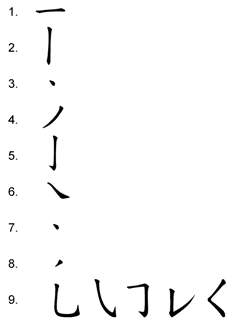
\includegraphics[scale=0.5]{chinese_strokes}
	\caption{A kínai karakterek alapvonásai}
	\label{fig:alapvonasok}
\end{figure}

Minden egyes vonásnak megvan a felépítési szabálya: az ecsetvonásoknak meghatározott sorrendben kell követniük egymást, még pedig általános elvként az írásjegyek határait alkotó virtuális négyszög bal felső sarkából lefelé és jobbra haladva. Az írásjegy gerincét, fő szerkezeti elemét adó nagyobb vonást, ha az egész írásjegyet átjárja, legutoljára húzzák.

\section{A vonássorrend szabályai}

Az előző szakaszban említett általános elv mellett az alábbi szabályokat alkalmazhatjuk az írásjegyek vonásainak sorrendjének meghatározásához.
\begin{enumerate}
	\item A vízszintes vonások megelőzik a függőleges vonásokat.
	\item A balra lejtő vonások megelőzik a jobbra lejtő vonásokat. 
	\item Az írásjegyek írását felülről kell kezdeni. 
	\item Az írásjegyet balról jobbra haladva építik fel. 
	\item A felülről keretezett írásjegyeknél előbb a keretet kell meghúzni. 
	\item Az alulról keretezett írásjegyeknél a keretet legvégül kell meghúzni. 
	\item A teljes keretet mindig legvégül kell bezárni.
\end{enumerate}

Egy szimmetrikus felépítésű írásjegynél előbb a középső részt kell kialakítani, s csak azután az oldalakat. Erre láthatunk egy példát \aref{fig:sorrend_pelda}. ábrán.

\begin{figure}[h]
	\centering
	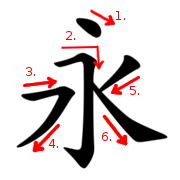
\includegraphics[scale=1.0]{images/vonasrend_ordered.png}
	\caption{Példa egy szimmetrikus írásjel vonásainak sorrendjére}
	\label{fig:sorrend_pelda}
\end{figure}

A kínai írásjegyek különböző számú alapvonásokból épülhetnek fel. Ezek közül a legegyszerűbb a csupán egyetlen vízszintes vonalból álló „egy” jelentésű \begin{CJK*}{UTF8}{gbsn}
一
\end{CJK*} ji írásjegy. A kínai írásrendszer más, egy vonásból álló írásjegyet nem tartalmaz. Aránylag ritkák a két vonásból álló írásjegyek is, például: \begin{CJK*}{UTF8}{gbsn}
二
\end{CJK*} er„kettő”,
\begin{CJK*}{UTF8}{gbsn}
十
\end{CJK*} si „tíz”,
\begin{CJK*}{UTF8}{gbsn}
人
\end{CJK*} zsen „ember” stb. A hagyományos írásjegyek zöme 15–30 vonásból épül fel (átlagosan 9 vonásból). Esetenként azonban ennél jóval több vonásból álló írásjegyek is előfordulhatnak, melyek tulajdonképpen már több önálló írásjegy összevonásának is tekinthetők. Ritkák ugyan, de léteznek 50 vagy akár 80 vonásból álló írásjegyek is.\Aref{fig:char_numbers} ábrán láthatjuk a karakterek mennyiségét stroke-ok száma szerint.

\begin{figure}[h]
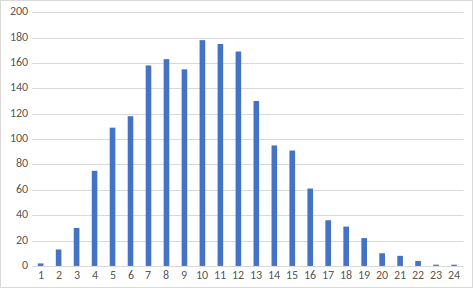
\includegraphics[scale=0.85]{images/chinese_char_by_strokes}
\centering
\caption{Kínai karakterek száma stroke-ok szerint}
\label{fig:char_numbers}
\end{figure}

\section{OCR megvalósítások}

\subsection{Az optikai karakterfelismerés feladata}

A különböző formátumú dokumentumok kezelésének egyik speciális esete, amikor a kezelendő dokumentumok még nem állnak rendelkezésre elektronikus formában. Ebben az esetben szinte mindig arról van szó, hogy a dokumentumok kinyomtatva, papír alapú hordozón jelennek meg. A későbbi feldolgozáshoz értelemszerűen digitalizálni kell a még nem digitalizált, papíron, nyomtatásban vagy írásban meglévő dokumentumokat, hogy az után elektronikusan szerkeszthető és feldolgozható legyen. Ebben a szituációban kap szerepet az optikai karakterfelismerés (\textit{Optical Character Recognition}, OCR). Az optikai karakterfelismerés a mesterséges intelligencia jelfeldolgozó és generalizációs képességeit kiaknázva képes nyomtatott, papír alapú dokumentumokon lévő karaktereket felismerni \cite{liu2013online}.

Az alap probléma itt az, hogy a nyomtatott, papír alapú dokumentumok esetében nagy zajaránnyal kell megküzdeni annak érdekében, hogy a releváns információt kinyerjük az érzékelt képi jelek és minták közül. Nyomtatott dokumentum esetében ilyen zajnak tekinthető például egy apró folt a papíron, tintaelmosódás, tintahiány, homályos háttér, apró gyűrődés a papíron, túl közeli vagy egybeolvadó betűk, betű dőlésszögének ingadozása stb. Kézírás esetén a kihívás még nagyobb, hiszen itt a személyiségjegyek sokszínűségéből adódó írásminták kavalkádjából kell megkűzdeni, hogy fel tudjuk imsertetni a karaktereket. Mind a nyomtatott, mind pedig a kézírásos esetben az optikai karakterfelismerő rendszer egy tanulási fázist követően képes olyan mintákat is osztályozni (a megfelelő karaktert felismerni), amelyekkel a tanulási fázisban nem találkozott, tehát megvan a szükséges generalizációs képessége.

Vannak készen elérhető OCR megoldások \cite{tmwebdvi77}, amelyek tipikusan az alábbi két részből állnak.
\begin{enumerate}
\item A szkennelő fejből, amely a dokumentum egészét vagy részeit beszkenneli. Hardverről van szó, ami elvégezi a digitalizálást. Két fizikai jelenségen alapszik fényvisszaverődésen és a fényelnyelésen.
\item  A mesterséges intelligencia szoftverből, ami elvégezi a beérkezett minták osztályozását, azaz magát a karakterfelismerést.
\end{enumerate}

\begin{figure}[h]
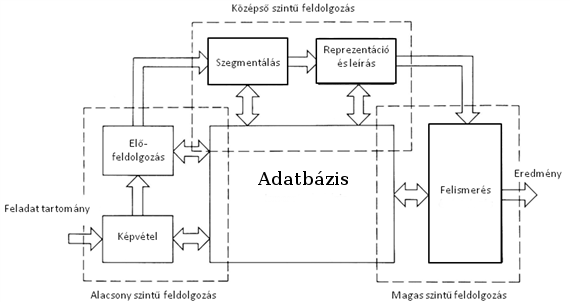
\includegraphics[scale=0.65]{images/ocr}
\centering
\caption{Az OCR-es feldolgozás szintjei}
\label{fig:feldolgozasi_szintek}
\end{figure}

Az OCR-el való feldolgozás során alapvetően három szintet \cite{feldolgozasi_szintek} különböztethetünk meg (\ref{fig:feldolgozasi_szintek}. ábra). 

\begin{enumerate}
\item Alacsony szintű (\textit{low-level}) feldolgozás
	\begin{itemize}
	\item A bemenet egy zajos kép, a kimenet pedig már egy tisztított, későbbi feldolgozásra alkalmasabb kép.
	\item Itt a kép minőségének a javításához az elterjedt képfeldolgozási előfeldolgozó algoritmusokat használják.
	\item Jellemző előfeldolgozások: \textit{zajszűrés, élesítés, finomítás, világosítás, maszkolás}.
	\end{itemize}
\item Középső szintű (\textit{intermediate-level}) feldolgozás
	\begin{itemize}
	\item A bemenetek képek, de a kiementek már a képekből nyert jellemzők.
	\item A kép komponenseinek kiemelése (szegmentálás) és azok jellemzése.
	\item Bizonyos mértékű mesterséges intelligencia/gépi tanulás szükséges hozzá.
	\end{itemize}
\item Magas szintű (\textit{high-level}) feldolgozás
	\begin{itemize}
	\item A felismert objektumok együttesének érzékelése (osztályozási probléma).
	\item Felismerés és értelmezés (interpretáció).
	\item Ezen a szinten kap kiemelt szerepet a mesterséges intelligencia módszereinek alkalmazása.
	\end{itemize}
\end{enumerate}

Az adatok kezelését struktúrált, ellenőrzött formában érdemes megoldani, amihez úgy általában egy adatbázis szükséges.

\begin{itemize}
\item A felismerni kivánt képek halmaza. A képekhez címkék tartoznak, ami szükséges a mesterséges intelligencia tanulás során.
\item A feldolgozott képek
	\begin{itemize}
	\item visszakerülnek az adatbázisba vagy
	\item továbbítják azt egy magasabb szintre
	\end{itemize}	  
\item Az interneten rengeteg adatbázis található: \textit{mnist, imagenet, kaggle, CASIA}
\end{itemize}

\subsection{Szegmentációs módszerek}

A szegmentáció során a karakterek közötti éles határ megtalálása a cél annak érdekében, hogy téves minták ne kerüljenek osztályozásra (például két fél karakter). A szegmentáció feladata lehet az is, hogy a karakter-dőlésszögeket, karakterméreteket normalizálja. Sok esetben a szöveges dokumentumokban nem csak karakterek vannak, hanem képek és egyéb, a felismerés szempontjából nem lényeges szimbólumok. A szegmentáció további feladata tehát az is, hogy az ilyen, számunkra nem releváns grafikus objektumok közül kiszűrje a csak karaktereket tartalmazó szöveges részeket. \Aref{fig:ocr_segmentation}. ábrán láthatunk egy példát arra, hogy hogyan képes az algoritmus kiemelni az egy karakterhez tartozó képrészt.

\begin{figure}[h]
\centering

\includegraphics[scale=1.0]{images/ocr_segmentation}
\caption{Példa egy név karaktereinek a szegmentálására}
\label{fig:ocr_segmentation}
{\cite{tmwebdvi77}}
\end{figure}


\subsection{Optikai előfeldolgozás}

Az előfeldolgozás a bemeneti minta komplexitásának csökkentésére szolgál, és annak legjellemzőbb vonásait emeli ki. Különösen nagy jelentősége van a kézírás felismerésekor, ugyanis az írott betűk jóval komplexebb mintákat alkothatnak, mint a nyomtatott betűk. A jellemzők kiemelése során a komplexitás úgy csökken, hogy közben a legjellemzőbb információk megmaradnak és ezáltal a későbbi feldolgozás számításigényét redukálhatjuk. Ez a folyamat tulajdonképpen egy komplexitáscsökkentéssel járó digitalizáció. \Aref{fig:ocr_preprocess}. ábra egy egyszerű digitalizálási módszert mutat, amikor az analóg jelre egy mátrixot reprezentáló rácshálót illesztünk, és amelyik cellán átmegy az analóg karakter, az az elem a mátrixban 1 értéket vesz fel (fekete), egyéb esetben pedig 0-t (fehér).

\begin{figure}[h]
\centering
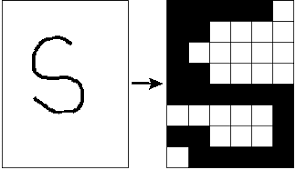
\includegraphics[scale=0.65]{images/ocr_preprocess}
\caption{Jellemzők kinyerésének egy fázisa, amely a dimenzió csökkenésével jár}
\label{fig:ocr_preprocess}
\end{figure}

\subsubsection{Dimenzió csökkentés}

A dimenziószám csökkentése optimálizálási folyamatnak tekinthető. A kivont jellemzőkben található redundáns információkat távolítja el. A tipikus dimenzió redukciós algoritmusok a gépi tanulás terén két részre oszthatók\cite{zhang2009patch}:
\begin{itemize}
\item hagyományos lineáris dimenziós redukció
	\begin{itemize}
	\item főkomponens-elemzés (PCA)\cite{gao2012dimensionality}: A PCA megpróbálja megtalálni egy olyan alteret, amelynek alapvektorai megfelelnek az eredeti tér maximális variancia irányainak.
	\item lineáris diszkriminancia-analízis (LDA)\cite{gao2012dimensionality}: Az LDA megtalálja azokat az irányokvektorokat, amelyek maximalizálják a különböző osztályok közötti szétválasztást (diszkriminánsát).
	\end{itemize}
\item tanulási alapú algoritmusok
	\begin{itemize}
	\item Helymegtartó előrejelzések (LPP)\cite{gao2012dimensionality}: Megőrzi a helyi kapcsolatokat az adatkészleten belül és feltárja az alapvető struktúráját. Az LPP egy felügyelet nélküli tanulási módszer, ami nem veszi figyelembe az osztálycímkét.
	\end{itemize}
\end{itemize}


\subsection{Felismerés}

Az osztályozás során történik meg a tényleges karakterfelismerés. A karakterfelismerő módszer a bemeneti jellemzővektor alapján dönti el, hogy az ismert karakterek közül melyikre hasonlít a legjobban a bemeneti vektor. Így a karakterfelismerési probléma egy asszociatív memóriát igénylő feladat, amelynek során a tárolt memóriaelemek közül kell előhívni azt, amely a bemeneti mintának legjobban megfelel.\\

\subsection{Kínai karakter felismerés}

A karakterek felismerése lehet online és offline karakterfelismerés. A fő különbség az, hogy az online karakterfelismerés rögzíti az ecsetvonások mozgását, míg az offline karakterfelismerés pusztán a karakter geometriai alakján alapul.

\begin{figure}[h]
\centering
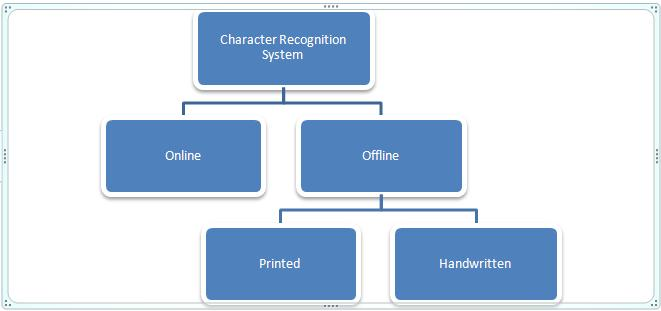
\includegraphics[scale=0.75]{images/ocr_online_offline}
\caption{Offline és Online Karakterfelismerés}
Forrás: \url{http://www.srimca.edu.in/Srijan/Srijanjan2011/IT/IntroductionToOCR.html}
\end{figure}

Az online karakterfelismerés során lehetőségünk van zaj generálására. Az ecsetvonások mozgása során véletlenszerű zajokat adhatunk hozzá. A zajos képekkel való betanítás a rendszerünk robusztusságát éri el.

Zaj hozzáadás:
\begin{itemize}
\item Pontszerű zajok: véletlenszerű fekete pixeltartomány hozzáadása
\item Elmosódások: Gauss elmosás alkalmazása
\item Forgatás: affin, perspektív transzformáció vagy forgatás origó körül 
\item Alacsony kontraszt: pixel megfelelő értékeinek szorzása
\end{itemize}

Az OCR folyamatba bevitt képek általában a szkennerekből származnak, amik képet és karaktert tartalmaznak. A karakterek gyakran különböző méretűek és betűtípusokat.

Az előfeldolgozás \cite{zhou2017stroke} során a következők jöhetnek szóba: 
\begin{itemize}
\item karakterek szétosztása a bemenetek függvényébe
\item a zaj megszüntetése
\item normalizálni a betűméretet és pozícionálni a filtert (kernel-t)
\item stroke váz generálása (thinning)
\end{itemize}

A jellemző alapú módszerek \cite{bunke1997handbook} kivonják a karakter jellemzőit, mivel ezek a jellemzők matematikailag számítottak, amire alkalmas számítógép. Így az optikai karakterfelismerés (OCR) nem igazán az optikai alapokon nyugszik, hanem inkább a matematikai számításokhoz köthető.

Amint említettem, minden kínai karakternek egyedi geometriai alakja van, amiket a stroke-ok alakítják (a stroke és az alapvonás színonim szavak). A kínai karakterek felismerésének alapja a stroke-ok és a strukturális jellemzők. Hosszú ideig ez a módszer befolyásolta a kínai karakterfelismerés kutatási irányát.
A karakter struktúrális lebontására láthatunk egy példát \aref{fig:ocr_features}. ábrán.

\begin{figure}[h]
\centering
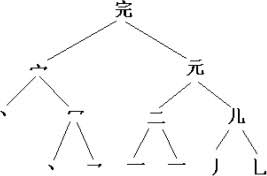
\includegraphics[scale=0.8]{images/ocr_features}
\caption{Egy kínai karakter lebontása alapelemekre, hogy az után azokat, mint jellemzőket lehessen használni}
\label{fig:ocr_features}
\end{figure}

Azonban ez nagyon nehéz a gyakorlatban, mert a stroke és a struktúrák közötti kapcsolat nagyon instabil. A stroke-ok és a strukturális jellemzők nem tudják hatékonyan kivonni a jellemzőket vagy nem praktikus.

Rengeteg mód van \cite{bunke1997handbook} a jellemzők kivonására, például lehet alapozni az él detektálásra, transzformációkra, rács jellemzőkre, kulcsfontosságú jellemzőkre, vektor vonali jellemzőkre.

Miután rendelkezésre állnak a módszerek, amikkel ki lehet nyerni a jellemzőket, hozzáfoghatunk a végleges kimenet előállítására. Lehetséges, hogy különböző felismerési rendszereket \cite{liu2013online} \cite{dong2005improved} \cite{zhong2015high} állíthat össze és összehasonlíthatjuk a kimeneteket. Azonban ez extra számítási költséget igényel, viszont a pontosság tovább javítható.

Mikor a felismerési rendszer kimenetet generál, lehetséges, hogy néhány karaktert tévesen osztályoz. Ez javítható a különböző bemeneti minták növelésével.

\subsection{Implementálás}

Egy olyan algoritmust \cite{wu2002recognition} mutatok be, ami képes kínai karakterek felismerésére sok különböző betűtípussal (pl. Song, Fang, Kai, Hei, Yuan, Lishu, Weibei és Xingkai). Ezekre a betűtípusokra \aref{fig:chinese_fonts}. ábrán láthatunk néhány példát.

Az algoritmus származtatott jellemzőkön alapul, és egy szótár halmazt használ. Először egy 3 szintes illesztést végez mindegyik szótárhoz képest. Az ilyen illesztésekhez kapcsolódó távolsági méréseket ezután egy központi diszkriminátorba táplálják, hogy a végső felismerési eredményt kiadják. Gyors és a pontos felismerést ért el mind a címben az összes 8 betűtípust és mind a főoldalon, amelyhez az első 4 általánosan használt betűtípus tartozik.

\begin{figure}[h]
\centering
\begin{tabular}{ c c }
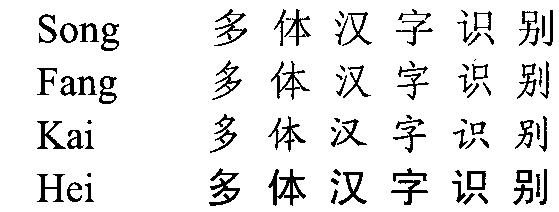
\includegraphics[scale=0.35]{images/chinese_fonts1} & 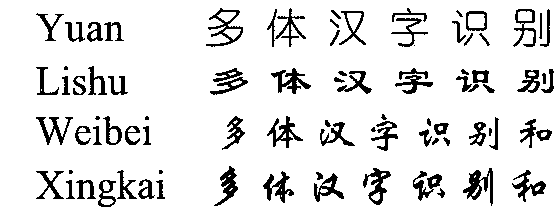
\includegraphics[scale=0.35]{images/chinese_fonts2}
\end{tabular}
\caption{Különféle kínai betűtípusok}
\label{fig:chinese_fonts}
\end{figure}

A funkciókivonás \cite{wu2002recognition} fontos eleme az OCR-nek. Az algoritmus egy 8-dimenziós vektor tartozik $[d_1, d_2, \ldots d_8]$. Kiszámítása az alábbi összefüggés segítségével történik
$$
d_i = \dfrac{l_i}{\sqrt{\displaystyle \sum_{k=1}^8 l_k^2}},
$$
ahol $i = 1, \ldots, 8$, és $l_i$ a csatlakoztatott fekete képpontok száma $i$-edik irányban. Erre egy példát láthatunk \aref{fig:8direction}. ábrán.

\begin{figure}[h]
\centering
\begin{tabular}{ c c }
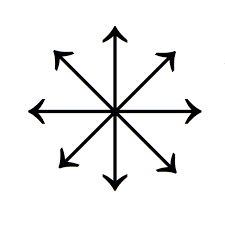
\includegraphics[scale=0.6]{images/8direction} & 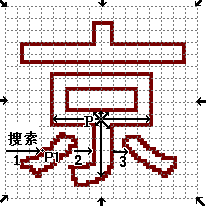
\includegraphics[scale=0.6]{images/ocr_PDC}
\end{tabular}
\caption{A jellemző irányok használati módja a karakterfelismerés során\cite{wu2002recognition}}
\label{fig:8direction}
\end{figure}

Az OCR rendszereknél, a felismerési algoritmusok két szakaszból állnak: tanítás és tesztelés. A hálózat súlyait a képzés során határozzák meg. A képzés után a rendszer átkapcsol a tesztelési fázisra, és a szótárak szerint meghatározza a legvalószínűbb karakterindexet.

A hierarchikus illeszkedés három szintből áll. Az első szint egy osztályozó, ami felhasználja a transzformált jellemzőket. Ezután a jellemzőket egy második szintű osztályozónak adják át. Az osztályozó több elemet is kiemel (kisebb számú kimenet). A harmadik szint az összes elemet használni fogja, a karaktert a végső felismerés eredményeként kiválasztja.

A 3 szintű hierarchikus struktúra nem csak csökkenti a számítási komplexitást, hanem figyelembe veszi a jellemzők összetevőit. Az utóbbi növeli felismerési pontosság. A 3-szintű struktúra hatékonysága a felismerési arány, a sebesség és a memória használat.

Minden tesztet két kínai mintán végzik, összesen 7510 karakterrel. Ezek az eredmények azt mutatják, hogy a 8 betűtípus átlagos felismerési aránya 99,32\% a képzési minták esetében, pedig 98,96\%. A betűtípusonként eredményeket \aref{tab:ccr_results}. táblázat foglalja össze.

\begin{table}
\centering
\begin{tabular}{ |c|c|c|c|c|c|c|c|c|c|}
\hline
Font & Song & Fang & Kai & Hei & Yuan & Lishu & Weibei & Xingkai & Average\\
\hline
Train & 99.82 & 99.64 & 99.81 & 99.57 & 98.77 & 98.75 & 99.35 & 98.82 & 99.32\\
\hline
Test & 99.71 & 99.50 & 99.80 & 99.09 & 98.43 & 98.15 & 98.78 & 98.19 & 98.96\\
\hline
\end{tabular}
\caption{Az elérhető karakterfelismerő rendszer hatékonysága különböző betűtípusok esetén}
\label{tab:ccr_results}
{\cite{wu2002recognition}}
\end{table}

A kísérleti eredmények azt mutatják, hogy a javasolt algoritmus képes gyorsan és pontosan felismerni a karaktereket akár 8 különböző betűtípussal is. Az algoritmus kiváló felismerési teljesítményt nyújt a 4 leggyakrabban használt betűtípusnál \cite{ccr}.

A kísérleti eredmények azt mutatják, hogy a javasolt algoritmus képes gyorsan és pontosan felismerni a karaktereket akár 8 különböző betűtípussal is. Az algoritmus kiváló felismerési teljesítményt nyújt a 4 leggyakrabban használt betűtípusnál \cite{wu2002recognition}.

\Chapter{Minták generálása}

\section{Tanító mintapontok előállítása}

A megvalósító neurális hálózat betanítása felügyelt tanulás módszerrel történik. A minták alapján történő tanulás lényege, hogy az eljárás során a be és kimeneti mintapárokból igyekszünk megfelelő ismereteket kinyerni és ezzel a rendszer viselkedését módosítani. A hálózat feladata, hogy megtanulja a rendelkezésre álló mintapont párok által reprezentált bemenet-kimenet leképezést. Ehhez elő kell állítani a megfelelő adathalmazt.

Az adathalmaz előállítása elött definiálni kell a rajzolás dinamikáját. A vonal kirajzolás sorrendje mellet fontos a vonal vastagsága is. Az kézírás ugyan sokat változott, de az alapjai megmaradtak. A stroke-ok vastagsága az ecset gyorsaságától, az ecsetre ható nyomás nagyságától függ. A megfelelően rajzolt vonalakat nagyon fontosnak tartják a kínaiak, mivel a kultúrájukhoz tartozik. A kalligráfia elárulhatja az ember nemét, korát, személyességét és így tovább.

\begin{center}

\includegraphics[scale=0.8]{calligraphy}
\end{center}

\subsection{Vonal vastagság}

A következőkben részletezném a vonal vastagság változását a stroke-ok rajzolásának függvényébe. 

\begin{itemize}
\item A stroke-ok vége elvékonyul, ezt a valóságban az ecset hirtelen felemelésével érik el. (\textit{Van néhány kivétel: right fally} 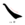
\includegraphics[scale=1.0]{right_fally}) 
\item Ha egy stroke végéből kezdődik egy másik stroke, akkor azok találkozásánál a vonalvastagság növekszik.
\item A horizontális vonalak közepe elvékonyul majd a végén újra vastagabb lesz. A vastagságot súlyokkal könnyedén lehet definiálni.

\begin{center}
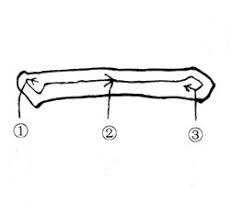
\includegraphics[scale=0.6]{horizontal_line}
\end{center}

\item A kampós vonalaknál (hooked stroke) a "kampó" hirtelen vékonyodással és irányváltoztatással jár. Az ecset hirtelen felemelésével érik el. Általában a kampó 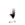
\includegraphics[scale=1.0]{hook} stroke része.
\item A további stroke-ok általában állandó vonal vastagsággal (ecset gyorsaság állandó). A kézzel írás és festés egyén függő.
\end{itemize}

\subsection{Környezet}
\begin{itemize}
\item A kínai karakterek festése papíron történik. A mi esetünkbe ez a képernyő. A karakterek fekete(0)-fehér(255) színüek. A szürke árnyalatokat [0,255] pixel értékek reprezentálják. A képernyő teljesen fehér, de a zaj generálásánál lehet hozzáadni fekete/szürke színt. 
\begin{lstlisting}[language=Python]
img = np.zeros((512, 512, 3), np.uint8)
img[0:512] = (255, 255, 255)
\end{lstlisting}
\item A festés alapvető eszköze az ecset. Az ecset lenyomássa egy ellipszis alakot hozz létre. A festés során az ecset elfordul (megfigyelésünk szerint 45fokban). Az ellipszis területe megnő, ha a festés gyorsasága csökken, ellenkező esetben csökken. Az ellipszist könnyedén lehet rajzolni OpenCV-be:
\begin{lstlisting}
cv2.ellipse(img, center, axes, angle, start_angle, 
	end_angle, color, thickness=1, lineType=8, shift=0) 
\end{lstlisting}
...
\end{itemize}

\subsection{Karakterek kirajzolása}
\begin{enumerate}
\item Poligonos közelítés: A kínai karakter ebben az esetben pontok halmaza és az ezeket összekötő poligonok. Minnél több ponttal definiáljuk a karaktert annál jobb minőségű képet érünk el, viszont a számítás igényünk növekszik.
\item Procedurális rajzolás: Ellipsziseket rajzolunk a képernyőre a kínai karakternek megfelelően. Az ellipsziseket érintő egyenesekkel összekötjük. Az ellipszisek tengelyeinek mérete különbözhetnek egymástól.
\begin{center}
\begin{tabular}{ c c }
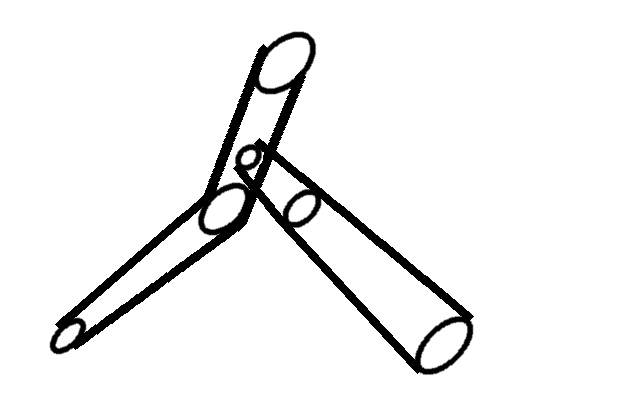
\includegraphics[scale=0.25]{proc_draw1} & 
\includegraphics[scale=0.5]{ren}
\end{tabular}
\end{center}
Az ellipszisek koordinátáit egy 5 dimenziós vektorral adhatjuk meg \(P_1 = (x_1, y_1, d_{x_1}, d_{y_1}, s_1)\) \(P_2 = (x_2, y_2, d_{x_2}, d_{y_2}, s_2)\). Az 'x' és 'y' koordináta párral az ellipszis középpontját adjuk meg. A $d_x$ és $d_y$ az ellipszis irányvektorai, amit majd a görbe kirajzolásnál lesz számunkra fontos. Az 's' az ellipszis területét adja meg. Meghatározza, hogy mennyire gyors az ecsetvonás (lassú->nagy terület, gyors->kis terület).
\begin{center}
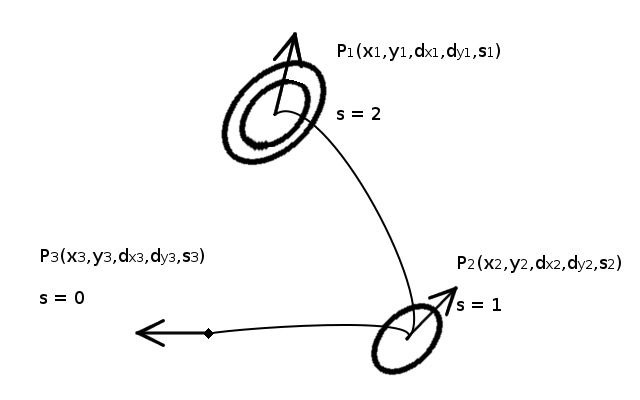
\includegraphics[scale=0.5]{image/proc_draw2}
\end{center}
\item Pontonkénti színszámítás: A képernyőt fellehet fogni mint egy n*m méretű mátix (képernyő szélessége: n, magassága: m). Az algoritmus pixelről pixelre haladva meghatározza annak értéket (0-255). A felbontás növekedés teljesítmény romláshoz vezet.
\end{enumerate}

A három karakter kirajzolás közül a procedurális rajzolás a legeffektívebb.

\subsection{Görbék}
\textit{Ide jöhet a Hermit}

\subsection{Karakter zajosítás}
\begin{itemize}
\item Pontszerű zajok
\item Elmosódások
\item Takarás
\item Vágás
\item Forgatás
\item Gyűrődés (textúrázás)
\item Alacsony kontraszt
\item Gradiens
\end{itemize}

\textit{Line break}\\\\

\begin{itemize}
\item Ecset dinamika
	\begin{itemize}
	\item \(P_1 = (x_1, y_1, d_{x_1}, d_{y_1}, s_1)\) \(P_2 = (x_2, y_2, d_{x_2}, d_{y_2}, s_2)\)
	\item Ecset szín (átmenetesség)
	\end{itemize}
\item Karakter kirajzolás
	\begin{itemize}
	\item Poligonos közelítés
	\item Procedurális rajzolás
	\item Pontonkénti színszámítás (fekete-szürke árnyalat-fehér)
	\item \textit{Görbék kirajzolása (Hermit)}
	\end{itemize}
\item Ideális karakter megjelenítés
\item Ideális karakter zajosítássa
	\begin{itemize}
	\item Különböző zajok
	\item Hálózat robosztussága
	\end{itemize}
\end{itemize}

\begin{comment}{Dolgozok a Hermit-es részen.}
\end{comment}

\begin{comment}{Ezek így vázlatnak jók, viszont az egyes pontokból legalább külön-külön szakaszoknak kellene majd lenni!}
\end{comment}

\Chapter{Neurális hálók}

A neurális hálózattokat \cite{neuralis77} gyakran hasonlítjuk az emberi agy működéséhez. Ha körültekintően szemügyre vesszük agyunk működését, akkor azt tapasztaljuk, hogy neuronokból és közöttük felépülő kapcsolatokból áll össze. A külvilágból érkezett ingereket értelmezhetjük úgy, mint egy bemenetet, amit az agyunkban lévő neuronok feldolgoznak.

A neurális hálózatokat gyakran hasonlítjuk az emberi agy működéséhez. Ha körültekintően szemügyre vesszük agyunk működését, akkor azt tapasztaljuk, hogy neuronokból és közöttük felépülő kapcsolatokból áll össze. A külvilágból érkezett ingereket értelmezhetjük úgy, mint egy bemenetet, amit az agyunkban lévő neuronok feldolgoznak.

\begin{figure}[h]
	\centering
	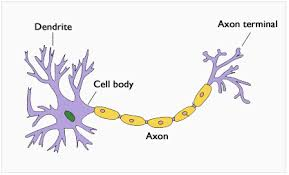
\includegraphics[scale=1.0]{images/neuron.png}
	\caption{A biológiai neuron fő részei}
	\label{fig:neuron}
	Forrás: \url{https://blog.vivekpanyam.com/deep-learning-made-simple-part-1/}
\end{figure}

A kutatók az agy felépítését vizsgálva egy olyan matematikai modellt dolgoztak ki, amely   reprezentálni próbálja az agyban található neuronokat  és a közöttük lévő kapcsolatokat. (Az agyban lévő neuron sematikus felépítését láthatjuk \aref{fig:neuron}. ábrán.) Ezt a modellt nevezzük neurális hálónak vagy neurális hálózatnak.

A neurális hálózatot alkotó neuronok úgynevezett rétegekbe rendeződnek. Háromféle réteget különbözetünk meg, a \textbf{\textit{bemeneti}}, a \textbf{\textit{kimeneti}} és a \textbf{\textit{rejtett réteget}}. Bemeneti és kimeneti rétegből minden hálózatban egy darab van, rejtett rétegből azonban tetszőleges számú lehet.

A hálózatban a rétegeket élek kötik össze egymással, amelyekhez egyenként egy-egy \textbf{\textit{súly}} tartozik. A neuronok a bemeneti éleiken kapott értékek és a súlyok segítségével bizonyos műveleteket végeznek el, majd az eredmény a kimeneti éleiken keresztül továbbítják a következő réteg neuronjai felé.

A tanítási folyamat elvégzésekor a hálózatba olyan bemenetet juttatunk, amelyhez tartozó kimenet ismert. A bemenetet végig futtatjuk a hálózat rétegein, majd a kimeneti réteg által szolgáltatott eredményt összehasonlítjuk a kimenet várt értékével. A két érték közötti eltérést a hálózat \textit{\textbf{hibájának}} nevezzük. A tanítás folyamán a hálózat súlyait úgy változtatjuk, hogy ez a hiba lehetőleg minél kisebb legyen. A hálózat betanítása után már olyan bemeneteket is megadhatunk, amelyeknek nem ismerjük a kimenetét, és a hálózat ezekre is képes hibahatáron belüli kimenetet produkálni.

\begin{figure}[h]
	\centering
	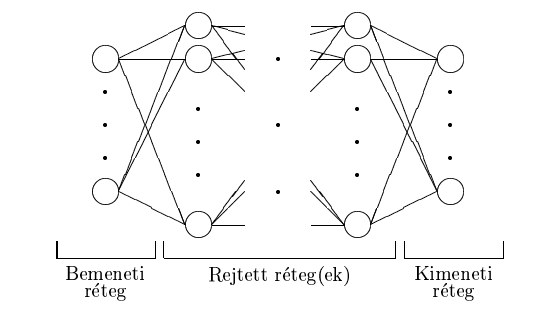
\includegraphics[scale=0.75]{images/ANNLayers.png}
	\caption{Egy általános felépítésű neurális hálózat\cite{neuralis77}}
\end{figure}

\section{A neurális hálók elemei}

Az egyszerűség kedvéért vizsgáljunk meg egy olyan neurális hálózatot, amelynek egyetlen neuronnal rendelkezik. Ezt szokás \textbf{\textit{Perceptron}}-nak is nevezni.

\textbf{\textit{Bemenet}}: Az kiértékelendő adat (ember számára ingerek), amit általában egy vektor (jelölje $x$) reprezentál.

\textit{\textbf{Súlyok}}: Két neuron közötti kapcsolat. Egy valós érték. A hálózat súlyait mátrixba tároljuk el (ezt jelölje $W$).

\textbf{\textit{Összegző csomópont}}: A bemeneteket összeszorozza a megfelelő súlyokkal és ezek összegét képezi. Tulajdonképpen mátrix szorzásról van szó.

$$
v(n) = \sum_{i=1}^{n}(w_ix_i)
$$

\textit{\textbf{Aktivációs függvény}}: Egy olyan függvény ($\varphi$), ami leképezi a kapott összeget egy adott intervallumba, amely általában a $[0, 1]$ vagy $[-1, 1]$ intervallumokat jelenti.

\textbf{\textit{Kimenet}}: A leképezett értékünk lesz a kimenetünk (jelölje $y$).

\begin{figure}[h]
	\centering
	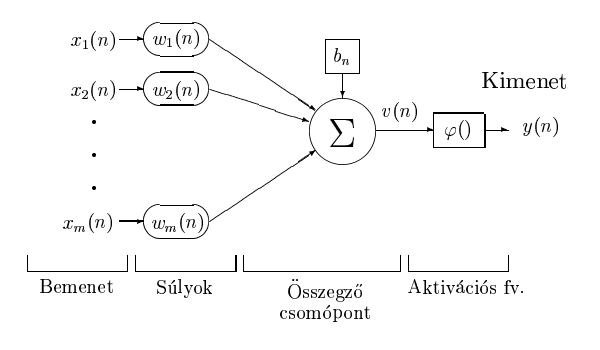
\includegraphics[scale=0.6]{images/ANNParts.png}
	\caption{A matematikai neuron modell felépítése\cite{neuralis77}}
	\label{fig:ANNParts}
\end{figure}

\Aref{fig:ANNParts}. ábrán láthatjuk a mesterséges neurális háló neuronjának matematikai modelljét. Ebben a $b_n$ változót \textit{bias}-nak nevezzük. A bias érték általában egy olyan bemenet, amely akkor is lehetővé teszi az $1$-es kimeneti értéket, ha a bemeneten $0$ érték szerepel. Ez kritikus fontoss-gú lehet a sikeres tanuláshoz. Tegyük fel hogy a neurális hálózat egy függvény: $y = mx$. A fenti függvény az origót metszi, ami nem minden esetben add jó eredményeket. A bias definiálásával a függvényünk kap egy konstans paramétert $y = mx + b$. A $b_n$-hez tartozó súly ($w_b$) általában -1 vagy 1.

Amennyiben az $x(n)$ bemenethez tartozó ideális kimenetet $d(n)$-nel jelöljük, illetve $y(n)$ jelenti a hálózat által az $x(n)$ bemenetre adott kimenetét, a neurális hálózat négyzetes hibáját a következőképpen értelmezzük:
$$
\varepsilon = (d(n) - y(n))^2.
$$

Ezt a hibát akarjuk a tanítási eljárás során minimálisra csökkenteni. Természetesen az lenne az ideális, ha a hibát egészen nullára tudnánk redukálni, de ez általában nem sikerül, ezért meg kell elégednünk egy kellően kicsiny hibaküszöbbel.

Aktivációs függvényként tetszőleges balról illetve jobbról folytonos eloszlásfüggvény megfelel, azaz olyan függvényt kell választanunk, amely
\begin{itemize}
\item monoton növekvő,
\item balról/jobbról folytonos,
\item határértéke $+\infty$-ben 1, $-\infty$ -ben 0.
\end{itemize}

Aktivációs függvénynek általában a szigmoid, azaz S alakú, függvényeket használjuk (mint például a logisztikus, tangens hiperbolikus függvények).

Az aktivációs függvényeknél egy úgynevezett rámpafüggvényről (RELU), ami az
$$
f(x) = max(0,x)
$$
összefüggéssel írható le, ahol $x$ az aktivációs függvény bemenete (\ref{fig:relu}. ábra).

\begin{figure}[h]
\centering
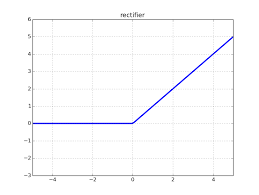
\includegraphics[scale=1.0]{images/relu}
\caption{A rámpafüggvény}
\label{fig:relu}
Forrás: \url{https://sefiks.com/2017/08/21/relu-as-neural-networks-activation-function/}
\end{figure}

A legújabb biológiai kutatások és a gyakorlati tapasztalatok is igazolják hogy a RELU-val történő tanítások szignifikánsan jobban teljesítenek. Legnagyobb előnye a regressziós tanítások esetén mutatkozik meg.

\section{A Backpropagation tanítási algoritmus}

Hiba minimalizálása során szükségünk van az aktuális hibára. Az összes kimeneti neuronra kiszámoljuk a négyzetes hibát és ezeket összeadjuk:
$$
E_{total} = \sum \dfrac{1}{2}(target - output)^2.
$$
(Az $\dfrac{1}{2}$ szorzót azért használjuk hogy el tudjuk távolítani majd a kitevőt a későbbiekben deriváláskor.)

A backpropagation célja, hogy frissítse az egyes súlyokat a hálózaton úgy, hogy az aktuális kimenet közelebb kerüljön a célkimenethez, ezáltal minimalizálva az egyes kimeneti neuronok és a hálózat egészének hibáját. A backpropagation algoritmus számításaira láthatunk egy példát \aref{fig:ANN_backprog}. ábrán.

\begin{figure}[h]
\centering
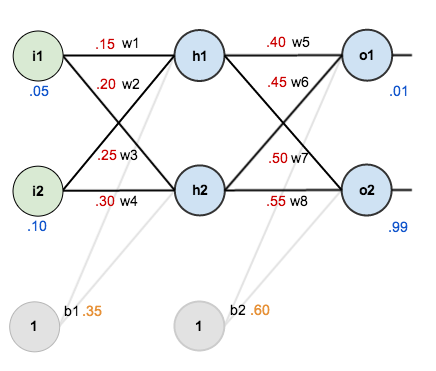
\includegraphics[scale=0.5]{images/ANN_backprog}
\caption{Példa a visszaterjesztéses tanítás alkalmazására}
Forrás: \url{https://mattmazur.com/2015/03/17/a-step-by-step-backpropagation-example/}
\label{fig:ANN_backprog}
\end{figure}

Tekintsük a $w_5$-öt. Azt szeretnénk tudni, hogy a $w_5$ változása milyen hatást gyakorol a teljes hibára, más néven $\frac{\partial E_ {total}}{\partial w_ {5}}$. Úgy is fogalmazhatunk hogy a gradiens a $w_5$ vonatkoztatásba.

Ezt a láncszabály alkalmazásával tudjuk kiszámolni:
$$
\frac{\partial E_{total}}{\partial w_{5}} = \frac{\partial E_{total}}{\partial out_{o1}} \cdot \frac{\partial out_{o1}}{\partial net_{o1}} \cdot \frac{\partial net_{o1}}{\partial w_{5}}.
$$

Lássuk az egyenlet elemeit!
\begin{flushleft}
\begin{equation}
E_{total} = \frac{1}{2}(target_{o1} - out_{o1})^{2} + \frac{1}{2}(target_{o2} - out_{o2})^{2}
\end{equation}
\begin{equation}
\frac{\partial E_{total}}{\partial out_{o1}} = 2 \cdot \frac{1}{2}(target_{o1} - out_{o1})^{2 - 1} \cdot (-1) + 0
\end{equation}
\begin{equation}
\frac{\partial E_{total}}{\partial out_{o1}} = -(target_{o1} - out_{o1}) = -(0.01 - 0.75136507) = 0.74136507
\end{equation}

\end{flushleft}

A logisztikus függvény parciális deriváltja a kimenet szorzata (1 - kimenet):
$$
out_{o1} = \frac{1}{1+e^{-net_{o1}}}
$$

$$
\frac{\partial out_{o1}}{\partial net_{o1}} = out_{o1}(1 - out_{o1}) = 0.75136507(1 - 0.75136507) = 0.186815602
$$

Végül, mennyire változik az $o1$ változó teljes bemenete a $w_5$ tekintetében?
$$
net_{o1} = w_5 \cdot out_{h1} + w_6 \cdot out_{h2} + b_2 \cdot 1
$$

$$
\frac{\partial net_{o1}}{\partial w_{5}} = 1 \cdot out_{h1} \cdot w_5^{(1 - 1)} + 0 + 0 = out_{h1} = 0.593269992
$$

Összesítve az eddigieket:
$$
\frac{\partial E_{total}}{\partial w_{5}} = \frac{\partial E_{total}}{\partial out_{o1}} \cdot \frac{\partial out_{o1}}{\partial net_{o1}} \cdot \frac{\partial net_{o1}}{\partial w_{5}}
$$

$$
\frac{\partial E_{total}}{\partial w_{5}} = 0.74136507 \cdot 0.186815602 \cdot 0.593269992 = 0.082167041
$$

A hiba csökkentése érdekében kivonjuk ezt az értéket az aktuális súlyból (adott esetben szorozva egy bizonyos tanulási sebességgel, $\eta$, amelyet 0,5-re állítunk):
$$
w_5^{+} = w_5 - \eta \cdot \frac{\partial E_{total}}{\partial w_{5}} = 0.4 - 0.5 \cdot 0.082167041 = 0.35891648
$$

Meg tudjuk ismételni ezt a folyamatot, hogy megkapjuk az új súlyokat $w_6$, $w_7$ és $w_8$:
$$
w_6 ^ {+} = 0,408666186
$$

$$
w_7 ^ {+} = 0.511301270
$$

$$
w_8 ^ {+} = 0.561370121
$$

Ezután folytatjuk a hátrafelé az új értékeket a $w_1$, $w_2$, $w_3$ és $w_4$ értékek kiszámításával. Hasonlóan láncszabályt alkalmazunk. A visszaterjesztés módjának egy szemléltetését \aref{fig:ANN_bp_viz}. ábrán láthatjuk.

\begin{figure}[h]
\centering
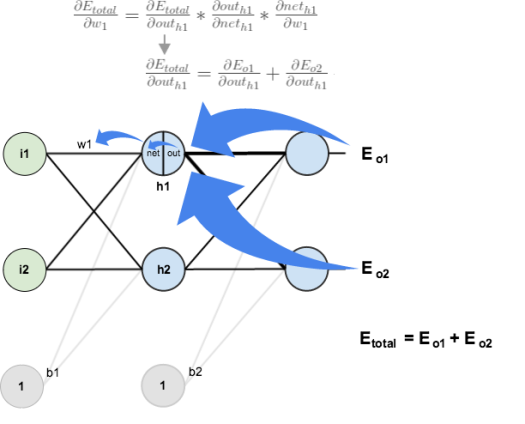
\includegraphics[scale=0.5]{images/ANN_bp_viz}
\caption{A hiba visszaterjesztése a súlyok módosításához}
\label{fig:ANN_bp_viz}
Forrás: \url{https://mattmazur.com/2015/03/17/a-step-by-step-backpropagation-example/}
\end{figure}

Végül frissítjük az összes súlyunkat. Amikor eredetileg a 0.05 és a 0.1 bemeneteket továbbítottuk, a hálózat hibája 0.2983711 volt. A backpropagation első fordulója után a teljes hiba 0.2910279 értékre csökken. Lehet, hogy nem tűnik soknak, de miután megismételtük ezt a folyamatot 10 000-szer, a hiba lecsökken 0.0000351-re.

\section{Konvolúciós neurális hálózat}

A konvolúciós neurális hálózat\cite{liconvolution}\cite{lecun1995convolutional} hagyományos neurális hálózat alapokon nyugszik. Annak egy speciális fajtája, amit képeken található minták feltárására fejlesztettek. Neuronokból épülnek fel és hasonlóképpen rendelkeznek tanítható súlyokkal. A bemeneteiken kapott értékek skaláris szorzatát egy nem lineáris leképezés követheti. Az egész hálózat reprezentálhat egy egyszerű osztályozó eljárást, aminek a bemenetei a nyers képpontok, és a kimenete lehet egy adott kép osztályba tartozás valószínűsége. A mi esetünkbe a bemenet a kínai karakter pixel értékei, a kimenet pedig valószíűségek a karakterekből adódóan.

A konvolúciós neurális hálózat hagyományos neurális hálózat alapokon nyugszik. Annak egy speciális fajtája, amit eredendően képeken található minták feltárására fejlesztettek. Neuronokból épülnek fel és hasonlóképpen rendelkeznek tanítható súlyokkal. A bemeneteiken kapott értékek skaláris szorzatát egy nem lineáris leképezés követheti. Az egész hálózat reprezentálhat egy egyszerű osztályozó eljárást, aminek a bemenetei a nyers képpontok, és a kimenete lehet egy adott kép osztályba tartozás valószínűsége. A mi esetünkben a bemenet a kínai karakterek pixel értékei, a kimenet pedig egy becsült osztályba tartozási mérték.

A hagyományos neurális hálózatok nem skálázzák a teljes képet. A kínai (különösen a hagyományos) több száz karaktert nem lehet megjeleníteni egy $16 \times 16$ pixeles rácsban. A megfelelő méret körülbelül $24 \times 24$ képpontot tartalmaz. Neurononként $24 \times 24 = 526$ súly paramétert jelentene. Ez még kezelhetőnek tűnik, de tisztán látszik, hogy a teljesen összekapcsolt struktúra nem kezeli jól a képeket.

Ha végig gondoljuk, hogy az hány paramétert jelent még egy kis neuronszámú kevés rejtett rétegből álló hálózat esetében, akkor rájöhetünk, hogy nagyobb méretű képen fellelhető minták felismeréséhez a hagyományos neurális hálózatok alkalmazása nem célravezető, emiatt a kép előfeldolgozására, szűrésére konvolúciós rétegeket vezetnek be.

\subsection{A háló felépítése}

A konvolúciós neurális hálózatokban szereplő rétegeket funkció alapján alapvetően két csoportra lehet bontani.

\begin{enumerate}
\item A konvolúciós rétegek, amik - mint paraméterezhető szűrők - előfeldolgozást végeznek a képen. Ezáltal a kép mérete lecsökken, a hordozott információtartalom kiemeltté válik.
\item A hagyományos neurális hálózat (második csoport) számára feldolgozható lesz, az osztályozást el tudja végezni. Egy konvolúciós neurális hálózat tehát konvolúciós és hagyományos rejtett rétegekből épül fel.
\end{enumerate}

A konvolúciós rétegek alapjában véve színes képek feldolgozására lettek kifejlesztve, ezért a neuronjaik három dimenzióban (szélesség, magasság, színcsatornák) vannak elrendezve.

A mi esetünkbe fekete-fehér képek állnak rendelkezésre. A színes képek esetén grayscale konvertálást végezhetünk el. Ha a pixel érték fekete akkor 0-át, ha fehér akkor 255-et rendelünk hozzá. A szürke árnyalatokat $[0, 255]$ közötti értékekkel definiáljuk. Egy kínai karakterre \aref{fig:chinese_char_pixel}. ábrán láthatunk példát.

\begin{figure}[h]
\centering
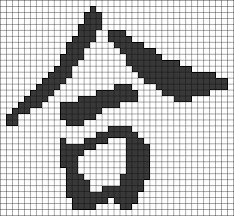
\includegraphics[scale=0.65]{images/chinese_char_pixel}
\caption{Egy kínai karakter fekete-fehér raszteres képként}
\label{fig:chinese_char_pixel}
\end{figure}

A következő felsorolásban - a tipikus, de nem kizárólagos sorrendre ügyelve - bemutatnám a konvolúciós hálózat rétegtípusait:

\begin{itemize}
\item \textit{Bemeneti réteg}: Tartalmazza a kép nyers pixel értékeit. Az értékeket sorba állítjuk és azokat egy 1 dimenziós vektor reprezentálja, ami 0 és 1 értékeket tartalmaz.

\item \textit{Konvolúciós réteg}: Adott képpont csoportokra konvolúció matematikai műveletet alkalmazunk. A konvolúció eredménye egy skalár (a skaláris szorzata a kép egy adott részének és a szűrőnek). Ha minden képpont csoportra elvégezzük a konvolúciót, akkor egy aktivációs térképet kapunk. Általában több szűrő paraméterrel is elvégezzük a konvolúciót és aktivációs térképeket egymásra rakjuk. Az aktivációs térkép, a művelet tulajdonsága miatt, kisebb
méretű lesz (\ref{fig:convolution}. ábra).

\begin{figure}[h]
\centering
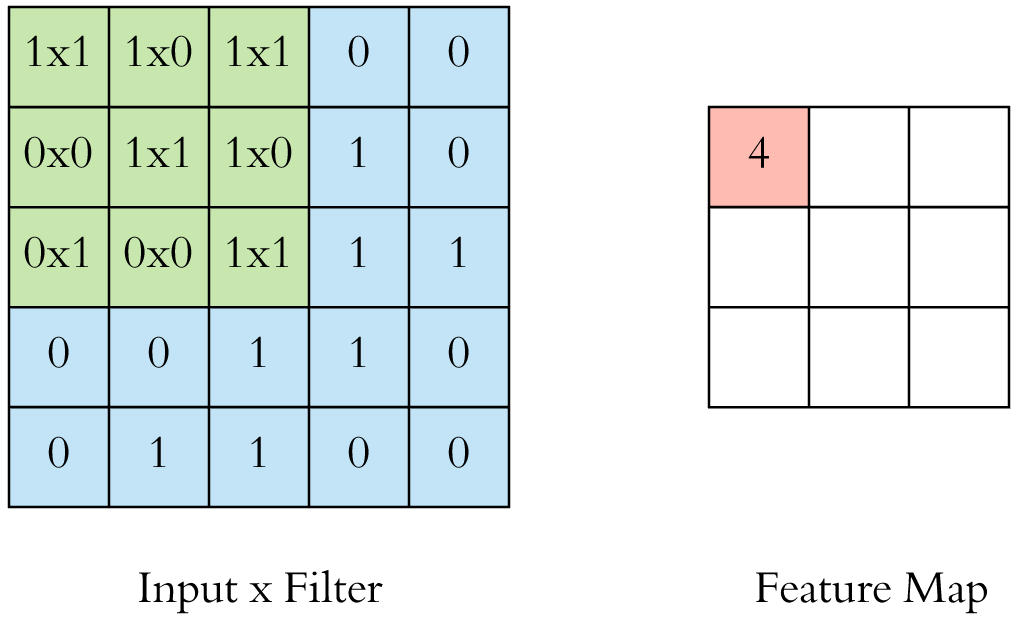
\includegraphics[scale=0.3]{images/convolution}
\caption{A bináris mátrix és a belőle konvolúcióval kinyert jellemzők}
Forrás: \url{https://towardsdatascience.com/applied-deep-learning-part-4-convolutional-neural-networks-584bc134c1e2}
\label{fig:convolution}
\end{figure}

Konkrétan mátrix szorzásról van szó. A feature map elemei egész számok, amik további konvolúciós rétegen mennek keresztül. Lehet közben különböző szűröket is használni.

A \textit{keras} Python csomagban ennek megvalósítása az alábbi módon lehetséges.
\begin{python}
from keras.models import Sequential
from keras.layers import Dense, Dropout, Flatten
from keras.layers import Conv2D, MaxPooling2D

model = Sequential()
model.add(Conv2D(64, (3, 3),
	weights=[np.random.normal(0, 0.01,
	size=(3, 3, 1, 64)), np.zeros(64)],
	activation='relu', padding='same',
	strides=(1, 1),
	input_shape=(1, 64, 64)))
\end{python}

\item \textit{RELU réteg}: A konvolúciós réteg aktivációs függvénye, ami a következő leképezést valósítja meg: $f(x) = max(x, 0)$. Vagyis, ha a bemenet kisebb, mint nulla, akkor a kimenet nulla lesz, ha nagyobb, mint nulla, akkor a kimenet a bemenet értékét veszi fel. A konvolúciós hálóknál a RELU sokkal gyorsabb más aktivációs függvényeknél, mint például a sigmoid vagy a tanh.
\item \textit{Összevonó réteg (pooling layer)}: A Pooling Layer függetlenül működik minden egyes feature map-nél. A MAX művelet segítségével kinyeri a legfontosabb vonásokat, csökkentve a dimenzióját. A leggyakoribb forma egy $2 \times 2$-es méretű szűrő, melyet 2 lépéssel kell felvinni minden szeletre. A bemenetben 2 szélesség és magasság mellett, az aktiválások 75\% -át eldobja. Minden MAX művelet ebben az esetben 4 számot vesz igénybe. Ennek használatát az alábbi kódpélda mutatja.
\begin{python}
model.add(MaxPooling2D(pool_size=(2, 2), strides=(2, 2)))
\end{python}

\begin{figure}[h]
\centering
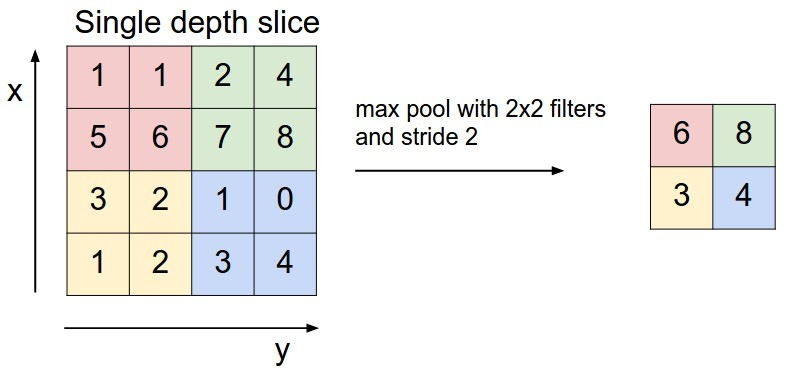
\includegraphics[scale=0.3]{images/maxpool}
\caption{A pooling réteg működése egy példán keresztül}
\label{fig:maxpool}
Forrás: \url{http://cs231n.github.io/convolutional-networks/}
\end{figure}

\item \textit{Teljesen összekötött réteg (fully connected, FC)}: Utolsó rétegekként szokták használni, hagyományos réteg. Lehet 1 vagy több réteg is a feladattól függően. Az osztályozás rész itt történik. A kimenetek valószínűségek a felsorolt karakterek szerint.
\begin{python}
model.add(Dense(200, activation='softmax'))
\end{python}
\end{itemize}

\Aref{fig:CNN_CCR_working}. ábra egy konvolúciós feldolgozást mutat be, ahol szemléltetve vannak az egyes rétegek utáni állapotok. A képen látható az egyes konvolúció utáni állapotok tulajdonság érzékelőként viselkednek.

\begin{figure}[h]
\centering
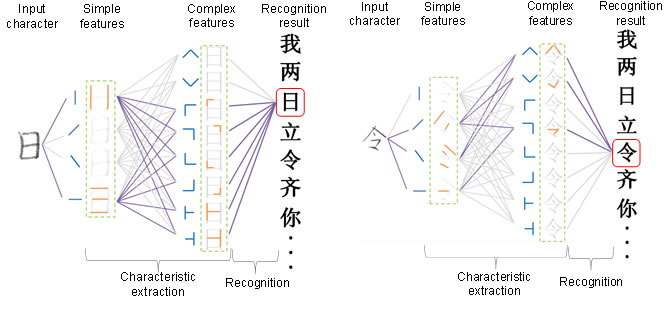
\includegraphics[scale=0.65]{images/CNN_CCR_working}
\caption{A konvolúciós karakterfelismerő hálózat sematikus felépítése}
Forrás: \url{http://www.fujitsu.com/global/Images/20130821-01b_tcm100-929717.jpg}
\label{fig:CNN_CCR_working}
\end{figure}

\subsection{Hálózat architektúra}

\begin{comment}{Melyik pontosan ez a cikk?}
\end{comment}

nagyon fontos a tervezés szakasznál. Egy 2013 kutatási papírt\cite{cirecsan2015multi} mutatnék be, miszerint a rétegek és a bennük lévő neuronok számával csökkenthető a hibaarány.

Először vessünk egy pillantást az adathalmazunkra. Az adat egyszerű képeket tartalmaz (offline kép). Tartalmaz 224419 karaktert, amelyeket 60 személy írt. A karakterek $48 \times 48$ pixelre skálázták. Az előfeldolgozás OpenCV-vel történik.

Nyolc hálózaton történt tanítás. Minden hálózatnak 11 rétege van, beleértve a bemeneti és kimeneti réteget. A jellemzők kinyerés fázisánál 100-450 darabszámú neuront használ. Végezetül két egymást követő teljesen összekötött (fully-connected) hálózat végzi el az osztályozást.

Tehát $48 \times 48$ bemeneti réteg, $xCy$ konvolúciós réteg, ahol $x$ neuronok (maps) száma és $y$ a szűrő mérete ($y \cdot y$). Az $MPy$ az összevonó réteg (max-pooling), ahol az $y$ a pooling méret ($y \cdot y$). Az $xN$ pedig a teljesen összekötött hálózat, ahol az $x$ a neuronok számát jelöli.

\begin{table}[h]
\centering
\caption{Forrás:\url{https://arxiv.org/pdf/1309.0261.pdf}}
\begin{tabular}{|l|l|l|}
\hline
 Háló &                                                                      & Hiba[\%] \\ \hline
0               & 48x48-150C3-MP2-250C2-MP2-350C2-MP2-450C2-MP2-1000N-3755N & 5.528 \\ \hline
1               & 48x48-150C3-MP2-250C2-MP2-350C2-MP2-450C2-MP2-1000N-3755N & 5.931 \\ \hline
2               & 48x48-300C3-MP2-300C2-MP2-300C2-MP2-300C2-MP2-1000N-3755N & 5.792 \\ \hline
3               & 48x48-100C3-MP2-200C2-MP2-300C2-MP2-400C2-MP2-500N-3755N  & 5.625 \\ \hline
4               & 48x48-100C3-MP2-200C2-MP2-300C2-MP2-400C2-MP2-1000N-3755N & 5.951 \\ \hline
5               & 48x48-100C3-MP2-200C2-MP2-300C2-MP2-400C2-MP2-1000N-3755N & 6.114 \\ \hline
6               & 48x48-100C3-MP2-200C2-MP2-300C2-MP2-400C2-MP2-1000N-3755N & 6.339 \\ \hline
7               & 48x48-100C3-MP2-200C2-MP2-300C2-MP2-400C2-MP2-500N-3755N  & 5.995 \\ \hline
\end{tabular}
\end{table}

Észrevehető, hogy a rétegekben a neuronok növelése csökkenti a hibaarányt. Bizonyítható, hogy a pontosság és a robusztusság növekszik, ha neuronok száma nő.

A bonyolult hálózatok gyakran hajlamosak a túltanulásra, overfitting-re. Az overfitting azt jelenti, hogy a hálózat túl jól illeszkedik a tanitó mintára, ezért az nem fog jól teljesíteni a teszt mintára.

Ilyenkor lehet kezdeményezni Dropout-ot, ami annyit jelent, hogy véletlenszerűen deaktivál neuronokat, hogy a hálózat más útvonalakon haladva máshogy fog tanulni. Ez Python-ban az alábbi kóddal valósítható meg.
\begin{python}
model.add(Dropout(0.5))
\end{python}

\begin{figure}[h]
\centering
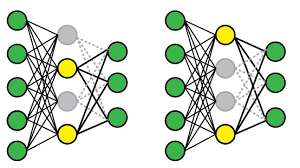
\includegraphics[scale=0.8]{images/dropout}
\caption{Neuronok véletlenszerű deaktiválása}
\label{fig:dropout}
\end{figure} 

\subsection{A háló tanítása}

Ez a neurális hálózatok egyik legfontosabb része. Sok kérdés merülhet fel olvasás közben. Hogyan ismerik az első konvolúciós rétegben lévő szűrők az élek és görbék keresését? Hogyan ismeri fel a teljesen összekapcsolt réteg a jellemzőket? Hogyan ismerik a szűrők az egyes rétegekben milyen értékeket kapnak? A számítógép képes beállítani a szűrő értékeit (vagy súlyait) a backpropagation-nek nevezett képzési folyamat révén.

Ez a neurális hálózatok használatának egyik lényeges pontja. Sok kérdés merülhet fel a megfelelő tanítási algoritmus kiválasztása közben.
\begin{itemize}
\item Hogyan ismerik az első konvolúciós rétegben lévő szűrők az élek és görbék keresését?
\item Hogyan ismeri fel a teljesen összekapcsolt réteg a jellemzőket?
\item Hogyan ismerik a szűrők az egyes rétegekben milyen értékeket kapnak?
\end{itemize}
A számítógép képes beállítani a szűrő értékeit (vagy súlyait) a backpropagation-nek nevezett eljárással.

A backpropagation\cite{ABeginne32} négy különböző szakaszra osztható
\begin{itemize}
\item Előre terjesztés (forward pass)
\item Veszteség számítás (loss function)
\item Hiba visszaterjesztés (backward pass)
\item Súly frissítés (weight update)
\end{itemize}

Az előre terjesztés során egy kínai karakter képét (amelynek mérete például $48 \times 48$ pixel) továbbítunk az egész hálózaton. Az első leképzésnél, mivel minden súly és szűrőérték véletlenszerűen van inicializálva, így a kimenet is valószínűleg véletlenszerű lesz, ezért a hálózat nem add pontos osztályozást. A hálózat jelenlegi súlyaival nem tudja keresni az alacsony szintű jellemzőket, ilyenek például a stroke-ok. Emiatt tovább lépünk a veszteség számítás részre. Ne felejtsük el, hogy a tanító mintának van egy címkéje. A veszteségfüggvény többféle módon definiálható, de gyakori az \textit{MSE} (\textit{Mean Squared Error}, átlagos négyzetes hiba)
$$
E_{total} = \sum 1/2(target - output)^2.
$$ 

A \textit{target} egy vektor, aminek az értékei azt mutatják meg, hogy az adott minta a neurális háló döntése alapján mennyire illeszkedik a megfelelő karakterre. Ezt tipikusan úgy állítják össze, hogy a $0$ jelentse azt, hogy egyáltalán nem illeszkedik, az $1$ érték pedig, hogy a háló döntése alapján az a karakter teljesen illeszkedik.

A modell használatát mutatja az alábbi kódrészlet.
\begin{python}
model.compile(loss='categorical_crossentropy',
              optimizer='adadelta',
              metrics=['accuracy'])
\end{python}

\begin{comment}{A képzési címke magyar nyelvű irodalomban szerepelt?}
\end{comment}

A veszteség rendkívül magas az első képzésnél. Olyan pontra akarunk jutni, ahol az előre jelzett címke megegyezik a képzési címkével. Ahhoz, hogy odaérjünk, minimálisra csökkentjük a veszteségünket. Azt szeretnénk megtudni, hogy mely bemenetek/súlyok azok, amelyek leginkább hozzájárultak a hálózat veszteségéhez (vagy hibájához). Ezt az illeszkedést az alábbi módon határozhatjuk meg.

\begin{python}
model.fit(f['trn/x'], f['trn/y'],	
	validation_data=(f['vld/x'], f['vld/y']),
	epochs=15, batch_size=128,
	shuffle='batch', verbose=1)
\end{python}

A négyzetes hibafüggvény szemléltetését láthatjuk \aref{fig:CNN_loss}. ábrán.

\begin{figure}[h]
\centering
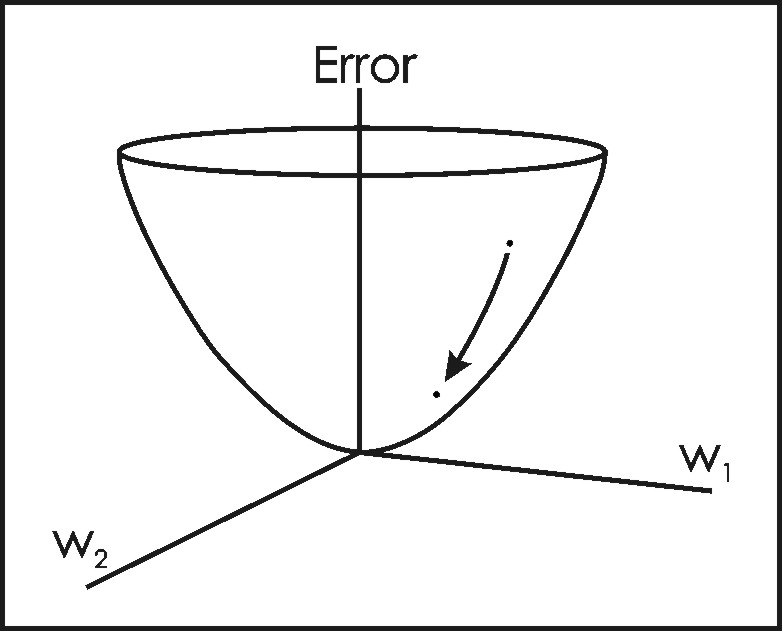
\includegraphics[scale=0.4]{images/CNN_loss}
\caption{A négyzetes hibafelület}
Forrás: \url{https://adeshpande3.github.io/A-Beginner%27s-Guide-To-Understanding-Convolutional-Neural-Networks/}
\label{fig:CNN_loss}
\end{figure}

A $dL/dW$ matematikai egyenlet írjuk fel a veszteség hozzájárulást. Következő lépés a hiba visszaterjesztés, amely meghatározza, hogy a súlyok milyen mértékben járultak hozzá a veszteséghez, és megtalálják azokat a módokat, amelyekkel a károk csökkenthetők. Miután kiszámítjuk ezt a származékot, akkor megyünk az utolsó lépéshez, amely a súlyok frissítése. Itt vesszük az összes súlyt és szűröt, és frissítjük őket úgy, hogy a gradiens ellenkező irányba változzon. Ekkor
$$
w = w_i - \eta \dfrac{dL}{dW},
$$
ahol $w$ a súly, a $w_i$ a kezdeti súly, az $\eta$ pedig a tanulási tényező.

A tanulási tényező egy olyan paraméter, amelyet a programozó választ. A magas tanulási arány azt jelenti, hogy nagyobb súlycsökkenést kell végrehajtani a súlycsökkentésekben, így kevesebb időre lehet szükség ahhoz, hogy a modell konvergáljon az optimális súlycsoporton. Azonban a túl magas tanulási arány olyan túl nagy ugrásokhoz vezethet, amelyek nem elég pontosak ahhoz, hogy elérjék az optimális pontot. Ennek egy szemléltetését láthatjuk \aref{fig:CNN_learning_rate}. ábrán.

\begin{figure}[h]
\centering
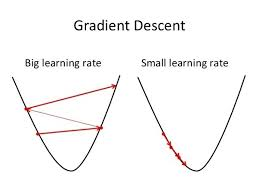
\includegraphics[scale=0.8]{images/CNN_learning_rate}
\caption{Magas és alacsony tanulási tényezők hatása}
Forrás: \url{https://adeshpande3.github.io/A-Beginner%27s-Guide-To-Understanding-Convolutional-Neural-Networks/}
\label{fig:CNN_learning_rate}
\end{figure}

Az előre terjesztés, a veszteség számítás, a visszaterjesztés és a paraméterfrissítés folyamata egy képzési iteráció. A program megismételi ezt a folyamatot egy rögzített számú iterációra. Miután befejezte a paraméter frissítést az utolsó képzésnél, remélhetőleg a hálózat megfelelően működik.

\subsection{Tesztelés}

Végül megnézzük, hogy működik-e a hálózat vagy sem. Különböző (még nem látott) képeket továbbíthatunk a CNN-en keresztül. Összehasonlítjuk a kimeneteket a címkékkel, és megnézzük a hibát. Ha alacsony hibát kapunk a hálózat jól dolgozott.

\subsection{Transfer learning}

A konvolúciós hálózatok betanításához nagyszámú mintára és nagy teljesítményű számítógépekre van szükség. Amennyiben nem áll rendelkezésünkre nagyjából egymillió képkockából álló tanító adathalmaz, akkor kis számú mintáról beszélünk. Ha nincs lehetőségünk vagy erőforrásunk nagy adathalmazzal tanítani, akkor is megvalósíthatjuk a kívánt leképezést. A transfer learning (tanulás átadása) módszer segítségével egy előre betanított hálózatot veszünk alapul, és annak utolsó pár rétegét lecserélve végezzük a tanítást. Ilyenkor a megmaradt rétegek betanított tulajdonság érzékelő funkciója segítségével a lecserélt rétegek által megvalósítandó leképezés könnyebbé vállhat. A konvolúciós neurális hálózatok tanítása esetében ez egy gyakori eljárás. A weben számos előre betanított hálózat található.

\begin{comment}{Az egész fejezetnek arról kell szólnia, hogy hogy lehetett a konvolúciós neurális hálót alkalmazni a konkrét, karakterfelismerési problémára. Az általános részeket ennek megfelelően érdemes lehet átírni, vagy csak egy rövid áttekintésnek tekinteni a fejezet elején.}
\end{comment}

\begin{comment}{Konkrét, OCR konvolúciós megoldások hivatkozásai is kellenének majd.}
\end{comment}

\Chapter{Validáció}

\begin{itemize}
\item Train/Test Data
	\begin{itemize}
	\item Train -> Betanítás
	\item Test -> Valídáció	
	\end{itemize}
\end{itemize}

\begin{itemize}
\item Paraméterek változtatása
	\begin{itemize}
	\item LR
	\item Filter
	\item Layers, Activation Func
	\item Neurons, Maps
	\item ....
	\end{itemize}
\item steps, epoch, batch computing...
\item Learning curve (gráf és magyarázat)
\end{itemize}

\begin{itemize}
\item hagyományos neurális hálózaton
\item konvoluciós neurális hálózaton
	\begin{itemize}
	\item Architektúra 1
	\item Architektúra 2
	\item Architektúra 3
	\end{itemize}
\end{itemize}
\Chapter{Összegzés}

A TDK dolgozatba betekintést nyertünk a kínai karakterek alap felépítésével. Továbbá megismerkedtünk azok építőelemeivel az alapvonásokkal (strokes). Dolgozatomba leírtam a vonásrendek szabályait, amely hasznos az online karakterfelismerésnél.

Részleteztem az optikai karakterfelismerés (OCR) müködését. Kifejtettem az optikai karakterfelismerés részeit. Bemutattam manapság használt OCR-t, amely képes felismerni a nyomtatott kínai karaktereket különböző betűtípuson. Táblázattal vizualizáltam a betűtípusok felismerésének pontosságát.\\

A minta generálás fontos eleme a rendszernek. A különböző mintákkal való betanítás a hálózatot robosztussá teszi. A széles körű zajok hozzáadása a képekhez, majd azzal való tanítás növeli a hálózat adaptációs képességét (zavaros képekre).

A stroke-ok kirajzolásának mechanikáját részleteztem. Megemlítettem a vonal vastagság fontosságát. Felvázoltam a vonal kirajzolás dinamikáját: pont paraméterei, vonal görbítésse Hermit ívek alkalmazásával. Továbbá bemutattam hogyan lehet openCV-vel zajokat hozzáadni a képekhez.\\

A neurális hálózat elemeivel megismerkedhetünk. A mögötte lévő matematikát megemlítettem és illusztratív képekkel probáltam megkönnyíteni a megértést.

Ezt követően a kép felismeréshez leghatékonyabb konvolúciós neurális hálózatot (CNN) részleteztem. Kifejtettem a CNN rétegeinek működését. Továbbá bemutattam egy kutatási cikket, amely a pontosságát hasonlítja össze különböző hálózat architektúrák szerint.\\

A valídáció során betekintést nyerhetünk, hogy hogyan változik a hálózat osztályozása a bemeneti képektől. Az adathalmazok előállítása után a hálózat betanítás következett. Végül a tesztelés során kiderült, hogy a teszt eredmények kapcsolatba vannak a tanító halmazzal.

% \Chapter{Irodalomjegyzék}
\begin{thebibliography}{9}
\addcontentsline{toc}{chapter}{Irodalomjegyzék}
% \addcontentsline{toc}{chapter}{Irodalomjegyzék}


\end{thebibliography}
 % 2

\end{document}

